\chapter{Einleitung}\label{ch:intro}

% Hinführung für Fachfremde: vom Allgemeinen (Suchbäume) zum Speziellen (Mess-System als Lösung),
% suchbaum-first.

\section{Motivation}\label{sec:motivation}
Suchbäume und Indexstrukturen tragen moderne datenintensive Systeme --- von In-Memory-Datenbanken über
Dateisysteme bis zur Sprachverarbeitung. Zugleich werden Prozessoren von der Speicher-Hierarchie
dominiert: nicht die Zahl der Operationen, sondern ihr Cache-Verhalten bestimmt die
Laufzeit~\cite{hennessy2019architecture, drepper2007memory, wulf1995memorywall}. Aus diesem
Spannungsfeld erwächst die Leitfrage der Arbeit.
Im Zentrum stehen dabei trie-basierte Indizes und cache-line-optimierte Verarbeitung. Seit dem
Adaptive Radix Tree (ART)~\cite{leis2013art} von 2013 hat sich die Forschung ausdifferenziert:
Trie-Höhen-Optimierung (HOT~\cite{binna2018hot}), hybride B\textsuperscript{+}-Strukturen
(Masstree~\cite{mao2012masstree}, B\textsuperscript{2}-Baum~\cite{schmeisser2022b2tree}),
hash-/trie-/B\textsuperscript{+}-hybride geordnete Indizes (Wormhole~\cite{wu2019wormhole}),
succinct-Repräsentationen
(CoCo-Trie~\cite{boffa2024coco}, SuRF~\cite{zhang2018surf}) und selbstoptimierende Ansätze
(START~\cite{fent2020start}).

\begin{figure}[htbp]\centering
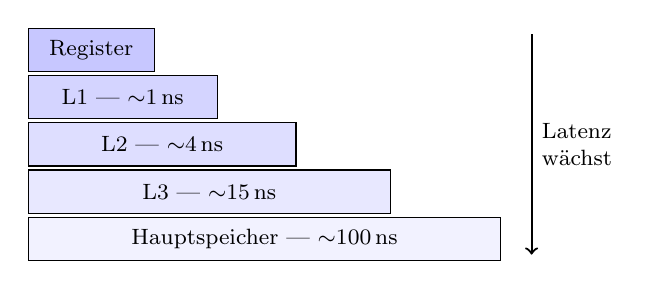
\begin{tikzpicture}[font=\footnotesize, lvl/.style={draw, minimum height=0.55cm, anchor=west, align=left}]
  \node[lvl, minimum width=1.6cm, fill=blue!22] at (0,2.0)  {Register};
  \node[lvl, minimum width=2.4cm, fill=blue!17] at (0,1.4)  {L1 --- $\sim$1\,ns};
  \node[lvl, minimum width=3.4cm, fill=blue!13] at (0,0.8)  {L2 --- $\sim$4\,ns};
  \node[lvl, minimum width=4.6cm, fill=blue!9]  at (0,0.2)  {L3 --- $\sim$15\,ns};
  \node[lvl, minimum width=6.0cm, fill=blue!5]  at (0,-0.4) {Hauptspeicher --- $\sim$100\,ns};
  \draw[->,thick] (6.4,2.2) -- (6.4,-0.6) node[midway,right,align=left]{Latenz\\wächst};
\end{tikzpicture}
\caption{Die \enquote{Cache-Wand}: typische Größenordnungen der Zugriffslatenz je Ebene der
Speicher-Hierarchie (Literaturwerte nach~\cite{hennessy2019architecture, drepper2007memory}); über die
Hierarchie wächst die Latenz um rund zwei Größenordnungen.}\label{fig:cache-wall}
\end{figure}

Parallel dazu ist ein eigener Forschungskorpus zu Cache-Bewusstheit, Prefetching und
Allokationsstrategien entstanden. Heuristiken wie Cache-Sensitive Search
Trees~\cite{rao1999css, rao2000csb}, cache-oblivious Layouts~\cite{frigo1999cache},
Prefetching-B\textsuperscript{+}-Bäume~\cite{chen2001prefetch} und hierarchisches
Prefetching~\cite{zhang2025hierarchical} adressieren jeweils einen separat betrachteten
Aspekt der Suchalgorithmus-Architektur, wobei der Fokus meist auf empirisch gefundenen Verbesserungen
und Messungen liegt. Weil so vieles auf cache-line-optimiertem Verhalten beruht, liegt eine
Segmentierung der Suchalgorithmus-Bestandteile in \emph{Achsen} nahe --- eine rückwärtsgerichtete
Abstraktion bekannter Bausteine in wiederverwendbare Module über die wichtigsten Arbeiten des Standes
der Technik hinweg.

Diese Arbeit vollzieht diese Segmentierung mit einem Rahmenwerk, dessen Bausteine sich als austauschbare
Entwurfsdimensionen eines großen Entwurfsraums (\emph{design space}) auffassen
lassen~\cite{idreos2018periodic, idreos2018datacalculator}. Strukturell
verschiedene Suchverfahren --- von baumartigen Indizes bis zu nicht-baumartigen Hash-Tabellen, samt
Spezialeigenschaften wie Cache-Line-Bewusstheit --- werden so als Punkte desselben Entwurfsraums vergleichbar;
nicht-baumartige Verfahren belegen dabei eine eingeschränkte Teilmenge (\emph{subset}) der Dimensionen
über demselben Suchalgorithmus-Interface, als wären sie der einzige Fächer einer Baum-Wurzel. Als
Prüfling für die Stand-der-Technik-Zugehörigkeit dient PRT-ART, ein Probst-Redirect-Tree-/ART-Hybrid und
eine abstrakte, unvollständige Ansammlung neuartiger Suchalgorithmus-Bestandteile.

\section{Problemstellung}\label{sec:problem}
Cache-Bewusstheit ist in heutigen Suchstrukturen entweder fest verdrahtet oder ganz ignoriert; vor allem
aber lässt sich nicht \emph{trennen}, welche einzelne Entwurfsentscheidung welchem Lastmuster nützt --- das
\emph{Trennbarkeits-Problem}, der rote Faden dieser Arbeit.

Bestehende cache-bewusste Index-Entwürfe optimieren ein oder wenige Aspekte isoliert und berichten
Ergebnisse, die sich über Veröffentlichungen hinweg schwer vergleichen lassen, da jede Arbeit eigene
Datenstrukturen, Workloads und Mess-Methodiken verwendet. Die Gewichtungen der Verbesserungen einzelner
Algorithmus-Bestandteile bleiben dabei untrennbar: Ein gemeldeter Leistungsgewinn lässt sich nicht
eindeutig auf einen einzelnen Bestandteil (Seitentyp, Layout, Value-Ablage, Prefetching) zurückführen,
weil die Bestandteile in den Original-Entwürfen verflochten bleiben. Es fehlt ein gemeinsamer Rahmen,
der (i)~solche Entwürfe in austauschbare Achsen zerlegt, (ii)~publizierte Algorithmen als explizite
Konfigurationen rekonstruiert und (iii)~sowohl einzelne Achsen als auch ganze Algorithmen auf einer
einheitlichen, fairen Basis vermessen kann.

\begin{figure}[htbp]\centering
\begin{tikzpicture}[font=\footnotesize, align=center, >=Stealth]
  \node[draw, fill=black!75, text=white, minimum width=2.4cm, minimum height=2.2cm] (mono) at (0,0){Algorithmus\\(Monolith)\\[1mm]{\Large ?}};
  \node[font=\scriptsize] at (0,-1.65){Welcher Teil hilft?};
  \draw[->,very thick] (1.5,0) -- (2.9,0);
  \node[draw, fill=green!12, minimum width=2.2cm] (a1) at (4.9,0.85){Knotentyp};
  \node[draw, fill=green!12, minimum width=2.2cm] (a2) at (4.9,0.0){Layout};
  \node[draw, fill=green!12, minimum width=2.2cm] (a3) at (4.9,-0.85){Allokator};
  \node[font=\scriptsize] at (4.9,-1.65){jede Achse einzeln messbar};
\end{tikzpicture}
\caption{Das Trennbarkeits-Problem: als Monolith bleibt unklar, welche Entwurfsentscheidung wirkt; erst die Zerlegung in orthogonale Achsen macht jeden Beitrag isoliert messbar.}\label{fig:separability}
\end{figure}

\section{Forschungsfragen}\label{sec:rqs}
Aus der Aufgabenstellung und dem Ziel der Cache-Line-Optimierung ergeben sich --- aufgrund der
Allgegenwärtigkeit des Einflusses der Cache-Line-Einstellungen --- eine Hauptfrage (FF0) und vier
messbare Forschungsfragen (FF1--FF4); ergänzende Aspekte sind ihnen als vertiefende \emph{Teilfragen} zugeordnet.
Quer zu allen fünf Fragen liegt eine Kategorisierungs-Frage, die diese Arbeit als Begriffsprägung
mitführt: Schon die Aufgabenstellung unterscheidet das Gemessene (die Entwurfsbestandteile des
Algorithmus), die Plattform, auf der gebaut und gemessen wird, und das Messen selbst. Ob sich die
Achsen des Entwurfsraums entlang dieser drei Belange sauber in \emph{Organ-Achsen} (die
austauschbaren Entwurfsbestandteile des Algorithmus), \emph{System-Achsen} (die Belange der Bau-
und Ziel-Plattform) und \emph{Mess-Achsen} (die Belange des Messens selbst) trennen lassen --- und
wie eine solche Trennung zu bewerkstelligen ist, falls sie in einem Entwurf noch nicht vorhanden
ist --- wird in dieser Arbeit als Frage ausgelegt; die Teilfragen sind darum entlang dieser drei
\emph{Achsen-Kategorien} benannt. Der Ist-Stand dazu ist eindeutig: die Arbeit legt die Dreiteilung als
drei getrennte Achsen-Register\footnote{Ein Achsen-Register ist das Verzeichnis der Achsen einer
  Kategorie samt der je Achse angebotenen Bausteine (im Code eine Registry).} an --- ein
Organ-Achsen-Register, ein System-Achsen-Register und ein
Mess-Achsen-Register --- und prüft ihre Tragfähigkeit; die Antworten entwickeln die
Kapitel~\ref{ch:measurement},~\ref{ch:impl} und~\ref{ch:eval}.
Jede Frage wird dabei an genau einer Stelle beantwortet: FF1 in Abschnitt~\ref{sec:axis-triad} und
Kapitel~\ref{ch:impl}, FF2 in Abschnitt~\ref{sec:measurement-system} und Kapitel~\ref{ch:eval}
(FF2.d in Abschnitt~\ref{sec:workload-basics-known} und Abschnitt~\ref{sec:eval-workloads}), FF3 in
Abschnitt~\ref{sec:prtart-demo} und Kapitel~\ref{ch:eval}, FF4 in
Abschnitt~\ref{sec:impl-system-axes} und Abschnitt~\ref{sec:impl-pipeline} (FF4.a);
Kapitel~\ref{ch:conclusion} zieht die Bilanz je Haupt- und
Teilfrage. Die Teilfragen tragen dazu die Kennungen FF0.E, FF1.a, FF1.b, FF2.a, FF2.b, FF2.c, FF2.d,
FF3.a, FF3.b, FF4.a und FF4.E.
\begin{description}
  %% OWNER-VORLAGE: OV-K1-01 --- der Klammerausdruck \enquote{(Hybrid-CPUs, Sapphire Rapids)} ist
  %% eingefrorener Owner-Wortlaut der Fragestellung (Scope-Freeze). Er bleibt unverändert; die
  %% Fußnote trägt den Ist-Stand der vermessenen Flotte nach. Widerspruch genügt.
  \item[FF0 (Hauptfrage)] Wie stark verbessern \emph{aktive, messgetriebene}\footnote{Messgetrieben
  heißt eine Entscheidung, die auf erhobenen Messwerten gründet und nicht auf festen Modellannahmen;
  statisch ausgelegt ist eine Variante, deren Entscheidung beim Entwurf fest vorgegeben wird.}
  cache-bewusste
  Entscheidungen --- Seitentyp, Speicher-Layout, Value-Ablage und Prefetching --- die Leistung
  trie-basierter Suchstrukturen gegenüber \emph{passiven, statisch ausgelegten} Varianten auf
  unterschiedlichen CPU-Plattformen (Hybrid-CPUs, Sapphire
  Rapids)?\footnote{Vermessene Flotte dieser Arbeit sind die drei registrierten
  Maschinen-Signaturen: prod1 (AMD Zen~5, Ryzen~9~9950X3D), prod2 (Intel Core i9-12900K, Alder Lake --- % chktex 29
  eine Hybrid-CPU mit P- und E-Kernen) und ein ODROID-Board mit Intel-Gracemont-Kernen. Die
  Server-Plattform Sapphire
  Rapids (ZIH-Knoten Barnard, Xeon~8470) ist in der Plattform-Erkennung angelegt, aber nicht Teil der
  Messreihen (n/a).}
  \emph{Erweiterung FF0.E (Achsen-Kategorien):} Lässt sich ein gemessener Gewinn überhaupt eindeutig
  zuordnen --- der Entwurfsentscheidung selbst (Organ), der Bau- und Ziel-Plattform (System) oder
  dem Mess-Aufbau (Mess) ---, und welche Trennung der Achsen-Kategorien ist dafür nötig?
  \item[FF1 (Komposition)] Wie lässt sich ein Suchalgorithmus-Entwurf kanonisch in orthogonale
  Achsen zerlegen und in einer Permutationsmatrix\footnote{Kanonisch heißt die Zerlegung, wenn jede
  Achse einen festen Platz in einer verbindlichen Reihenfolge hat. Die Permutationsmatrix ist die
  Tabelle dieser Achsen mit ihren zulässigen Belegungen; jede Wahl genau einer Belegung je Achse ist
  eine Achsen-Permutation, und ein Profil ist die deklarative Beschreibung (als XML) eines Entwurfs
  durch seine Belegung dieser Achsen. Bias-frei heißt: ohne Verzerrung durch eine Nachimplementierung
  oder durch ungleiche Messbedingungen.} systematisieren, sodass die
  Stand-der-Technik-Verfahren möglichst aus ihrem Originalcode bias-frei als Profile
  rekonstruierbar und beliebig permutierbar werden? \emph{Teilfrage FF1.a (Kategorien-Schnitt):} Zerfällt
  die kanonische Zerlegung selbst entlang der drei Achsen-Kategorien --- müssen Plattform- und
  Mess-Belange aus der Permutationsmatrix herausgehalten werden, damit die Zerlegung der
  Entwurfsbestandteile orthogonal bleibt ---, und wie ist ein solcher Schnitt zu bewerkstelligen,
  falls er im Entwurf noch nicht angelegt ist? \emph{Teilfrage FF1.b (Organ-Kopplungen und
  System-Variation):} Welche wechselseitigen Abhängigkeiten zwischen Achsen (Knotentyp $\times$ SIMD
  $\times$ Pfadkompression)\footnote{SIMD (\emph{single instruction, multiple data}) bezeichnet
  Befehle, die eine Operation auf mehrere Datenelemente zugleich anwenden; die Pfadkompression fasst
  in einem Trie Knotenfolgen ohne Verzweigung zu einem Knoten zusammen; die ISA (\emph{instruction
  set architecture}) ist der Befehlssatz der Ziel-CPU, und SSE2/AVX2/AVX-512, NEON/SVE2 und RVV sind
  die SIMD-Erweiterungen der Befehlssätze x86, ARM und RISC-V\@.}
  begrenzen die Isolation einzelner Achsen, und wie verhält sich dieselbe Organ-Belegung
  im Cache-Update- und Cache-Line-Füllverhalten (wie der Cache aktualisiert wird und wie vollständig
  die geladenen Cache-Lines genutzt werden), wenn allein die ISA-/SIMD-Achse (SSE2/AVX2/AVX-512,
  NEON/SVE2, RVV) variiert wird --- soweit die jeweilige Zielplattform zum Bau freigegeben ist
  (Abschnitt~\ref{sec:axis-triad})?
  \item[FF2 (Mess-Methodik)] Wie muss eine reproduzierbare Mess-Pipeline mit
  Hardware-Zähler-Erhebung\footnote{Die Mess-Pipeline ist die Kette aus Bau der Binaries, Messlauf
  und Auswertung; Hardware-Zähler sind die Leistungszähler der CPU (\emph{Performance Monitoring
  Counter}, PMC), die Ereignisse wie Cache-Fehlzugriffe je Lauf zählen.} gestaltet sein, damit jede
  Achsen-Permutation fair (unter sonst gleichen
  Bedingungen, also gleicher Compiler- und Flag-Basis) in drei Messreihen --- A (Prüfling vs.\ Stand der
  Technik), B (systematische Variation der Entwurfsentscheidungen) und C (Merge/Regression
  alt gegen neu) --- über drei Granularitäten (Mikro-, Makro- und Gesamt-Benchmarking: einzelne
  Bestandteile, Interface-Operationen, ganze Algorithmen) gemessen wird, und unter welchen
  plattform-kalibrierten Kriterien (Schwellen, die je Maschinen-Signatur aus Messläufen auf der
  jeweiligen Plattform bestimmt werden) gilt eine Plattform als erfolgreich verifiziert?
  \emph{Teilfrage FF2.a (Mess-Achsen):} Müssen die Mess-Instrumente selbst --- Zeitnahme,
  Zähler-Erhebung, Last-Erzeugung --- als eigene Achsen geführt werden, die stets präsent sind,
  ohne je zu verändern, was gebaut und gemessen wird, und wie ist diese Trennung zu
  bewerkstelligen, falls sie noch nicht vorhanden ist?
  \emph{Teilfrage FF2.b (Organ-Achsen):} Wie lassen sich widersprüchliche Literaturbefunde zur optimalen
  Knoten-/Cache-Line-Größe (eine Cache-Line bei CSS/CSB\textsuperscript{+}~\cite{rao1999css, rao2000csb}
  gegenüber sechzehn und mehr bei Hankins/Patel~\cite{hankins2003nodesize}, dort Knoten von 512 Byte und
  größer bei 32-Byte-Cache-Lines, sowie mehrere, per Prefetch gemeinsam geladene Cache-Lines je Knoten
  bei den Prefetching-B\textsuperscript{+}-Bäumen von Chen, Gibbons und Mowry~\cite{chen2001prefetch})
  durch achsen-isolierte, unter
  sonst gleichen Bedingungen permutierte Messung
  bias-frei nachmessen, statt sie aus inkompatiblen Original-Setups zu übernehmen?
  \emph{Teilfrage FF2.c (Erweiterbarkeit):} Wie erweiterbar ist eine solche Mess-Pipeline --- wie
  gliedern sich neue Prüflinge und ihre Entwurfsbestandteile ein, wie werden sie abstrahiert, und
  ordnen sie sich bestehenden Gattungen\footnote{Gattung heißt in dieser Arbeit die oberste
  Einteilung der Algorithmen nach ihrem nach außen sichtbaren Interface (etwa \texttt{Map} oder
  \texttt{Container}); jede Gattung trägt ihre eigenen Unterklassen mit festem Achsensatz.} zu,
  begründen sie neue Gattungen oder eine
  Mischform; auf welcher konzeptionellen Ebene sollte dieser Schnitt verlaufen? Zentral ist dabei:
  Was ist überhaupt eine Erweiterung des Systems, und wie wirkt sich das Hinzufügen oder
  Wegschneiden einzelner Entwurfsbestandteile --- etwa derjenigen, die aus einer einzelnen
  Veröffentlichung stammen --- auf das erreichbare Maß an Cache-Line-Bewusstheit des
  Gesamtsystems aus? Braucht es
  dafür einen Betriebsmodus, der die Entwurfsbestandteile eines wählbaren Referenzentwurfs aus der
  Literatur als geschlossene Achsenmenge isoliert anbietet, um genau diese eine Veröffentlichung
  --- bei weiterhin freistehenden Mess- und System-Achsen --- originalgetreu durchzumessen?
  \emph{Teilfrage FF2.d (Workload-Stand der Technik):} Welche Workloads gehören gerade für
  Suchalgorithmen zum Stand der Technik?
  \item[FF3 (Prüfling-Vergleich)] Gewinnt der Prüfling PRT-ART gegenüber den acht Rang-1-Entwürfen
  im Stand der Technik (\emph{State of the Art}, kurz SOTA\@; ART, HOT, Masstree, CoCo-Trie, START,
  B\textsuperscript{2}-Baum, Wormhole,
  SuRF)\footnote{Die \emph{Ränge} ordnen die Stand-der-Technik-Veröffentlichungen nach Zentralität für diese Arbeit: Rang-1 umfasst die zehn wichtigsten Kern-Arbeiten --- darunter die acht eigenständigen Suchentwürfe sowie ARTSync (P08)~\cite{leis2016olc} und LOUDS (P09)~\cite{jacobson1989louds}, die als Organe eingehen ---, Rang-2 die cache-bewussten Layout- und B\textsuperscript{+}-Vorarbeiten und Rang-3 die Prefetching-, Synchronisations- und TU-Dresden-Hardware-Arbeiten.}
  und der Rang-2/3-SOTA \emph{nicht} durch asymptotische Neuheit, sondern durch bessere
  Mikroarchitektur-Eigenschaften\footnote{Die Cache-Line-Auslastung ist der Anteil der genutzten
  Bytes einer geladenen Cache-Line; LLC ist der Last-Level-Cache, die letzte Cache-Stufe vor dem
  Hauptspeicher; der dTLB (\emph{data translation lookaside buffer}) puffert Adressübersetzungen für
  Datenzugriffe; ein Miss ist ein Fehlzugriff, der die nächste, langsamere Stufe bemüht; Branch-Kosten
  sind die Kosten von Sprungbefehlen, vor allem falsch vorhergesagter Verzweigungen.} --- höhere
  Cache-Line-Auslastung, weniger LLC- und dTLB-Misses, geringere Branch-Kosten, kleinere heiße
  Suchpfade (die häufig durchlaufenen Knotenfolgen) --- bei Punktsuche, Prefix-Lookup (Suche nach
  einem Schlüssel-Präfix) und Prefix-Enumeration (Aufzählung aller Schlüssel zu einem Präfix),
  gemessen unter den drei Pflicht-Messreihen A (Prüfling vs.\ Stand der
  Technik), B (systematische Variation der Entwurfsentscheidungen) und C (Merge/Regression alt gegen
  neu)? \emph{Teilfrage FF3.a (Organ-Achsen):} Welche lokale Seitendarstellung (8-/16-Bit-Punktseite ---
  die Direktindex-Seiten Array$_{256}$ und Array$_{65535}$ --- gegenüber der Kompaktseite --- den
  Vektor-Seiten Vector$\langle$u8,u8$\rangle$ und Vector$\langle$u16,u16$\rangle$) ist je
  Verzweigungspunkt (je Knoten, an dem sich der Suchpfad verzweigt) am günstigsten, und nach welchen
  plattform-kalibrierten
  Umschaltregeln --- einschließlich der Reihenfolge
  Array$_{256}\to$Array$_{65535}\to$Vector$\langle$u8,u8$\rangle\to$Vector$\langle$u16,u16$\rangle$
  je Belegungsdichte und Zugriffsart --- soll adaptiv gewechselt werden? Der Prüfling schaltet derzeit nach festen
  Dichte-Schwellen von 25, 50 und 75~Prozent\footnote{Punktseite und Kompaktseite sind die zwei
  Seitenformen des PRT-ART-B\textsuperscript{+}-Knotens: Die Punktseite adressiert Einträge direkt über ein Feld mit 8-
  oder 16-Bit-Index, die Kompaktseite hält sortierte Schlüssel-Wert-Vektoren. Die Dichte-Schwellen
  sind die Umschaltregeln des Prüflings zwischen den Seitendarstellungen; die im Glossar genannte
  Grenze bei 50~Prozent ist die Seitentyp-Grenze zwischen Punkt- und Kompaktseite, keine weitere
  Umschaltregel.} um (Abschnitt~\ref{sec:prtart-demo}).
  \emph{Teilfrage FF3.b (Compile-Time-Zwang):} Erzwingen latenz-kritische Messungen, dass an sich zur
  Laufzeit wählbare Entscheidungen --- etwa solche adaptiven Umschaltregeln --- bereits zur
  Übersetzungszeit als Anforderungen fixiert werden, sodass sich jede Achse in eine
  übersetzungszeit-fixierte Haupt-Achse und laufzeit-variable Unter-Achsen
  gliedert --- eine Zuspitzung, die FF4 aufnimmt?
  \item[FF4 (Compile-Time vs.\ Laufzeit)] Welche Achsen-Eigenschaften müssen zur Übersetzungszeit
  fixiert werden, um plattform-optimierte, provenienz-nachweisbare\footnote{Provenienz-nachweisbar
  heißt: Die Herkunft einer Binary --- welche Achsen-Belegung, welche Plattform und welche
  Werkzeugkette sie hervorgebracht haben --- ist an der Binary selbst nachprüfbar. Dazu trägt jede
  Binary zwei Identitäten: die Binary-Identität je Permutation, also ihre Belegung der Organ-Achsen
  (im Code die \texttt{binary\_id}, ein Pfad aus einem Segment je Achse mit umkehrbar eindeutiger
  Zahlencodierung), und die Übersetzungszeit-Identität, die zusätzlich Bau-Plattform, Werkzeugkette,
  Bau-Steuergrößen und Quellstand umfasst und als Fingerprint --- ein Hash über alle
  bau-bestimmenden Glieder --- in die Binary einkompiliert wird; die erste heißt auch
  Permutations-Identität.} Binaries je Permutation zu
  erzeugen, und welche können bzw.\ müssen zur Laufzeit gewählt werden (bit-codierte
  Binary-Identität je Permutation, laufzeit-adaptive Layout-Wahl), ohne die wissenschaftliche
  Vergleichbarkeit (gleiche Compiler- und Flag-Basis) zu verletzen? Wird es durch die Messung möglich,
  ISA+OS-optimierte Binaries für eine Suchalgorithmus-Rekombination zu erzeugen, deren heuristische
  Optimierung perfekt auf ihre Laufzeitumgebung zugeschnitten ist?
  \emph{Teilfrage FF4.a (deklarative Kette):} Lässt sich der gesamte Ablauf --- vom plattformbezogenen
  Bau aller Binary-Permutationen der Entwurfsbestandteile über den Messlauf und die Auswahl der besten
  gemessenen Binary oder Binary-Rekombination bis zur Auswertung in CSV-/xlsx-Dateien, LaTeX und
  Diagrammen --- durchgehend aus einer XML-Beschreibung des Experiments erzeugen, sodass ein
  Experiment vollständig und reproduzierbar durch seine Deklaration bestimmt ist?
  \emph{Erweiterung FF4.E (System-Achsen):} Verläuft die Grenze zwischen Übersetzungszeit und Laufzeit
  entlang der Achsen-Kategorien --- gehören insbesondere die Plattform-Eigenschaften (ISA,
  Betriebssystem, Erweiterungs-Hardware wie GPU-, FPGA- oder NPU-Beschleuniger) als System-Belange in
  die Übersetzungszeit-Identität der
  Binary --- also in ihren Fingerprint, ohne die Permutations-Identität zu verändern ---, während
  Mess-Wahlen (die Belegungen der Mess-Achsen) laufzeit-variabel bleiben dürfen?
\end{description}

\section{Zielsetzung und Beiträge}\label{sec:contributions}
Die Zielsetzung folgt der Aufgabenstellung in vier Schritten: cache-bewusste Suchalgorithmen in
austauschbare Entwurfsbestandteile zerlegen, Stand-der-Technik-Entwürfe als explizite Konfigurationen
rekonstruieren, cache-line-bewusstes Verhalten sowohl je Bestandteil als auch für den ganzen Algorithmus
auf gemeinsamer CPU-only-Basis messen und auswerten sowie den besten Gesamtalgorithmus nach einer autonomen
Heuristik-Profil-Auswertung und Heuristik-Funktions-Modellierung als eigenständige Binary ausliefern.
Der Code der Diplomarbeit ist dabei der \emph{formale Konsument und Treiber} der Cache-Engine: Er lädt den
Prüfling PRT-ART, kompiliert ihn per Metaprogrammierung gegen die Kernbestandteile der Cache-Engine, liefert
ABI-stabile \emph{Lebewesen} (Suchalgorithmus-Instanzen) aus und treibt sie über das Prüf-Dock --- das
Mess-Interface der Gattung (Kapitel~\ref{ch:measurement}) --- zur Messung.
Das zugrunde liegende Architekturmodell
--- die drei Ebenen (\emph{Gattung} als äußeres Algorithmus-Interface, \emph{Gattungs-Unterklasse} mit
festem Achsen-Satz, im Code die Tier-Unterklasse \texttt{AnatomyGenus}, und die
Achsen-Or\-ga\-ne), die vier Subsysteme und die ABI-stabile Auslieferung der Suchalgorithmus-\emph{Lebewesen}
--- entwickeln
Kapitel~\ref{ch:measurement} und Kapitel~\ref{ch:impl}. Gemeint sind dabei die vier Träger-Subsysteme
Mess-Treiber, \texttt{CacheEngineBuilder}, \texttt{CacheEngine} und Prüfling; davon zu unterscheiden sind
die zwölf Stufen der Empfehlungs-Pipeline im Code. Das Konzept der Achsen-Architektur selbst ist aus einer
Vorarbeit des Autors übernommen --- dem Achsen-Konzept der UltiHash-Vorarbeit (zur Herkunft siehe
Abschnitt~\ref{sec:anatomy-patterns}) ---, der Beitrag dieser Arbeit ist
seine Übertragung auf cache-bewusste Suchstrukturen und seine mess-orientierte Realisierung. Die
zentralen Beiträge sind:
\begin{itemize}
  \item Eine ABI-stabile Modul-Schnittstelle: eine einheitliche C-Modulgrenze
  (\texttt{comdare\_\allowbreak{}create\_anatomy()} $\to$ \texttt{IAnatomyBase}) exportiert je
  Permutation genau ein Lebewesen; dahinter liegt eine dreischichtige Abstraktionskette --- eine
  Vermittlungs-Fassade (\texttt{ICacheEngine}) über der Laufzeit-ABI-Schicht
  (\texttt{IAnatomyBase} $\to$ \texttt{IExecutionEngine}) über den Achsen-Organen. Der Schnitt des
  Suchmaschinen-Moduls ist konzeptionell festgelegt, als eigenes Modul aber noch nicht vollzogen; sein
  Provider ist ausdrücklich zurückgestellt, und das Suchmaschinen-Modul lebt derzeit als
  Topic-Namensraum innerhalb der Cache-Engine. Der Prüfling-Suchkern spezialisiert seine Hybrid-API variadisch nach
  Parameterzahl (1~Parameter $\Rightarrow$ \texttt{std::vector}-API\@;
  2~Parameter $\Rightarrow$ \texttt{std::map}-API\@; $N>2 \Rightarrow$
  \texttt{std::map<K,\,std::tuple<V$_1$\ldots V$_N$>>}), wie es die Aufgabenstellung über alle Varianten
  der bekannten \texttt{std::map}- und \texttt{std::vector}-Container-Hüllen fordert; die Cache-Engine
  trägt dazu die Gattungs-Aritäten ihrer Gattungs-Unterklassen.
  \item Eine Achsen-Permutationsmatrix in dreigeteilter Ordnung: achtzehn Organ-Haupt-Achsen in fester
  Slot-Reihenfolge (T00--T17) tragen die Binary-Permutation; drei System-Haupt-Achsen --- Ziel-ISA,
  Betriebssystem und Erweiterungs-Hardware --- beschreiben die Bau- und Ziel-Plattform, wobei ihre
  Komplex-Klammer \texttt{build\_target\_complex} ausdrücklich keine vierte Haupt-Achse ist; und ein
  eigenständiger Mess-Achsen-Realm hält die Mess-Belange von beidem getrennt, denn weder System- noch
  Mess-Achsen gehen je in die Permutations-Identität der Binary ein. Eine optionale neunzehnte
  Organ-Achse für Festplatten-IO, deren Beschreibung selbst beschrieben wird, tritt hinzu, sobald
  Platten-IO in den Algorithmus-Entwurf eingebunden wird; sie stempelt im Klammer-Anhang der
  Organ-Zeile und bleibt außerhalb der Permutations-Identität. Umgesetzt ist die Matrix mit Boost.MP11-Compile-Time-Typlisten-Bausteinen ---
  Laufzeit-Tags und \texttt{std::variant} sind in den Tier-Binaries als Doktrin verboten
  (\texttt{[[no-runtime-switch]]}) --- samt Compile-Time-Fallback zwischen Prüfling-Stack und
  Stand-der-Technik-Stack, der sechzehn der achtzehn Achsen aus dem Cache-Engine-Rahmen übernimmt und
  zwei durch Prüfling-Slots ersetzt.
  \item Dreiunddreißig Stand-der-Technik-Profile als persistierte XML-Konfigurationen (P01--P33):
  30~Vollprofile eigenständiger Suchentwürfe --- 8~Rang-1 und 22~Rang-2/3 --- sowie 3~abstrakte Profile
  (OLC, LOUDS, VAMPIR), die nur seziert als Organe bzw.\ Mess-Technologie eingehen. Der
  \texttt{ExperimentDriver} überführt sie automatisch in vorkompilierte C++23-Module; der Profilsatz
  deckt damit alle 33 analysierten Veröffentlichungen ab. Der XML-Entwurf bildet mithilfe der
  Cache-Engine die einzelnen Algorithmus-Bestandteile zur Kompilierzeit echt ab und ist damit eine
  Compiler-Compiler-Bauanleitung in einem modellgetriebenen Optimierungs-Stack
  (\emph{model-driven})~\cite{schmidt2006modeldriven}; dass deklarative Konfigurationsbeschreibungen den
  automatisierten Aufbau modularer Systemvarianten steuern, ist ein etabliertes
  Konstrukt~\cite{czarnecki2000generative, apel2013feature}.
  \item PRT-ART als Prüfling mit acht eigenen Bausteinschichten (4+1+2-Pool-Allokator, optimistisches
  Lock-Coupling mit reservierten Blöcken, MultiLevel-Layout, pfadorientiertes Prefetch,
  DensityTracker, Hypothesen-Metriken H1/H2/H3, Inline/External/ChainRef-ValueHandles,
  Signaling-Bit-Serialisierung). Im Mess-Apparat meldet der Prüfling vier Prüfling-Slots an --- Seitentyp
  (\texttt{page\_type}, in der Cache-Engine die Achse \texttt{node\_type}), Prefetch, Telemetrie und den
  ChainRef-Value-Handle --- sowie ein Merge-Organ für die Pfadkompression, das die Cache-Engine-eigene
  Patricia-Strategie trägt; im codegen-fähigen Mess-Pfad wirken davon derzeit zwei (Prefetch und
  Value-Handle), während MultiLevel-Layout, Pool-Allokator und Serialisierung über den
  Cache-Engine-Standard laufen (Abschnitt~\ref{sec:prtart-demo}). Die Telemetrie ist in der Cache-Engine
  eine System-Achse und kein Kompositions-Slot; der gleichnamige Prüfling-Slot ist ein
  Bestandsrest. Die OLC-Nebenläufigkeit ist eine Bausteinschicht des Prüflings, kein angemeldeter Slot.
  Zu beachten ist, dass die Slot-Nummern des Prüflings nicht der Slot-Reihenfolge T00--T17 der
  Cache-Engine folgen. Der Einsatz des Prüflings zeigt die Erweiterbarkeit des Systems am Beispiel ---
  zur effizienten Weiterentwicklung neuartiger Ansätze im Umgang mit cache-aware Algorithmen und
  beschleunigter Suche.
  \item Ein Mess-Treiber mit Defined-/Full-Modus-Unterscheidung (ergänzt um eine deterministisch
  gestichprobte Full-Variante), profilbewusstem Workload-Routing --- im Standard die Voll-Permutation über alle registrierten Workloads, deren Durchführungsstand
  Kapitel~\ref{ch:eval} ausweist --- und drei Granularitäten: Mikro-, Makro- und Gesamt-Benchmarking
  (einzelne Bestandteile, Interface-Operationen, ganze Algorithmen).
  \item Eine durchgehend deklarativ gesteuerte Bau- und Mess-Kette hinter diesem Treiber: ein
  Experiment-\emph{Planer} löst die XML-Beschreibung des Experiments gegen die Achsen-Angebote der
  drei Achsen-Register auf, und der \texttt{CacheEngineBuilder} baut und vermisst daraus
  plattformbezogen die Binary-Permutationen --- bis zur Auswertung über die xlsx-Ausgabe (die Mappe
  ist Ausgabe und Standard; die CSV-Form ist kein einzelnes Kind-Dokument, sondern ein geordneter Baum aus
  CSV-Dateien --- ein Gesamtordner je Mappe, darunter ein Ordner je Blatt, darin die CSV-Dateien der
  einzelnen Unter-Achsen-Fahrten ---, der immer aus der Mappe erzeugt wird, als Strategie derselben Factory,
  und per XML statt der Mappe oder zusätzlich zu ihr am selben Ziel liegt) und die daraus erzeugten
  LaTeX-Tabellen und TikZ-Diagramme.
  \item Eine bias-freie Vergleichs-Matrix, die \emph{alle} registrierten Lastprofile gegen \emph{alle}
  rekonstruierten Lebewesen fährt --- die aus den Profil-XML gebauten Original-Entwurfs-Binaries --- und
  so der Selbstbevorzugung durch autor-eigene Mess-Aufbauten in Einzelveröffentlichungen begegnet
  (englischer Musterbegriff: \emph{home-field advantage})~\cite{vanderkouwe2019benchmarking}.
  \item Eine generische Plattform-Probe, die die Cache-Eigenschaften je Zielplattform ermittelt ---
  Line-Größe und Größen je Hierarchie-Ebene aus sysfs und CPUID --- und als feste Größen in eine
  systemoptimierte Binary einfließen lässt. Die Kern-Topologie (P-/E-Kern-Trennung, Pinning) ist als
  Plattform-Belang derselben Probe vorgesehen und für die Cache-Line-Messung auf Hybrid-CPUs Pflicht,
  ihre Erfassung ist im vorliegenden Stand jedoch bewusst ungesetzt --- der Durchführungsstand steht in
  Kapitel~\ref{ch:eval}. Die beiden Produktionsmaschinen sollen unter zwei Betriebssystemen
  (immutables Talos und root-Linux mit vollem Hardware-Zähler-Zugriff) vermessen werden --- zur
  Abgabe liegt das root-Linux-Regime vor, der Talos-Spiegel steht aus.
  \item \emph{Als Zielsetzung und Ausblick:} die Auslieferung und begründete Auswertung des besten
  Gesamtalgorithmus --- automatisch ausgewählt aus den feingliedrigen Messergebnissen unter dem
  Messaspekt des besten cache-bewussten Verhaltens und der Beschleunigung durch Cache-Line-Anpassung, im
  Vergleich aller messbaren Parameter gegen die Binary-Wettbewerber --- als eigenständige, ABI-stabile
  Binary hinter dem einheitlichen Suchalgorithmus-Interface. Die Mess-Pipeline liefert die dafür
  nötige Rangbildung bereits, und ein erstes Inkrement der automatischen Auswahl und des
  Binary-Versands ist als eigenständiges Werkzeug (\texttt{best\_binary\_selector}) implementiert;
  die heuristik-gesteuerte Vollautomatisierung bleibt Ausblick.
\end{itemize}

\section{Aufbau der Arbeit}\label{sec:structure}
Der Aufbau folgt dem Weg vom Allgemeinen zum Speziellen: Kapitel~\ref{ch:foundations} legt --- konzeptionell und
bildhaft --- die Grundlagen aus bekanntem Wissen: die Landschaft der Suchstrukturen, die
Hardware-Eigenschaften der Speicherhierarchie, die Workload-Konventionen der Vergleichsliteratur, die
Software-Mittel der Abstraktion und den Heuristik-Begriff. Kapitel~\ref{ch:measurement} entwickelt
daraus die Konzepte eines cache-bewussten Mess-Systems: die Problemstellung und ihre Anforderungen, den
Stand der Technik als Achsen-Instanzen, das Anatomie-Modell mit seinen Schichten, das Mess-System
selbst, den Prüfling PRT-ART als Demonstrator und die heuristische Auswertung samt ihrer
Betriebsmodi. Kapitel~\ref{ch:impl} setzt dieses Konzept als Software-Architektur um --- Repositorien,
der Prüfling im Code, Achsen-Architektur und Übersetzungs-Pipeline, Schichten-Verträge mit
Contract-Tests sowie die System-Achsen im Code. Kapitel~\ref{ch:eval} wertet entlang der
Forschungsfragen aus, einschließlich des heuristischen Gegenbeweises; Kapitel~\ref{ch:conclusion}
schließt mit Fazit und Ausblick. Die Anhänge vertiefen begleitend: die Messreihen-Dokumentation (Anhang~\ref{app:measurements}),
die Code-Struktur (Anhang~\ref{app:code}), das Glossar (Anhang~\ref{app:glossary}), die vollständige
Bausteine-Matrix (Anhang~\ref{app:blocks}), die Architekturentscheidungen (Anhang~\ref{app:adr}) und die
Vergleichs-Interfaces (Anhang~\ref{app:interfaces}).
